%
At leading order, the modelling of the signal kinematic is expected to be independent from the model parameters. To verify this assumption dedicated test samples 
were produced corresponding to tan$\beta$=1, 5, 10, 20. Figure~\ref{fig:tan_beta_dep_1} shows an example of comparison between a subset of these test samples generated 
with $m_{H}=~1$~TeV; there are no observable differences between samples using different tan$\beta$ values.  

\begin{figure}[htbp]
  \begin{center}\setlength{\tabcolsep}{2.0pt}\small   
    \begin{tabular}{cc}
      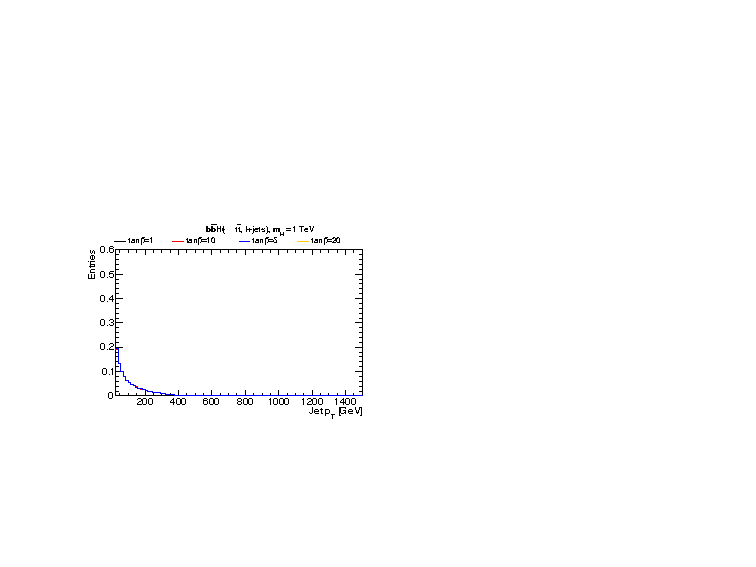
\includegraphics[width=0.47\textwidth]{figures/signal_modeling/tanbeta/fig_1_tanbeta.pdf} &
      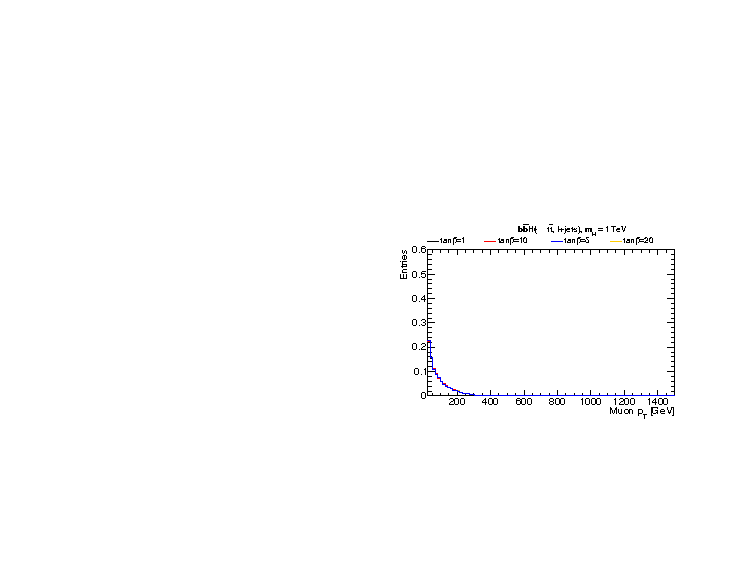
\includegraphics[width=0.47\textwidth]{figures/signal_modeling/tanbeta/fig_2_tanbeta.pdf} \\
     \end{tabular}
     \caption{Comparison of jet \pt\ (left) and muon \pt\ (right) for signal test samples generated with $m_{H}=~1$~TeV and different tan$\beta$ values as described in the text.}
   \label{fig:tan_beta_dep_1}
  \end{center}
\end{figure}
